\chapter{Estado del Arte}
\label{chapter:Estado del Arte}

Una de las aplicaciones más comunes dentro de la detección de anomalías es para la detección de intrusos (\textit{Intrusion Detection}) y la creación de sistemas de detección de intrusos (\textit{Intrusion Detection System, IDS}). Se trata de sistemas cuyo objetivo es la monitorización de los sistemas y redes informáticas, con el fin de alertar en caso de que puedan existir brechas de seguridad\cite{intrusionSystems}. 

Con la ingente cantidad de redes y sistemas que se pueden encontrar a día de hoy es necesario incluir uno de estos sistemas, con el fin de mantener la integridad y disponibilidad de los mismos. Dentro de los IDS, se pueden identificar dos grandes implementaciones de estos sistemas, en los sistemas de detección de intrusos en Host (\textit{Host-Based Intrusion Detection Systems, HIDS}) y los sistemas de detección de intrusos en red (\textit{Network Intrusion Detection Systems, NIDS}).

\begin{itemize}
    \item \textbf{HIDS:} Estos sistemas se caracterizan por implementarse en el Host utilizando información del propio sistema operativo para detectar actos maliciosos \cite{HIDS}. Esta información tiene distintos niveles de información, pero por lo general tienden a ser de bajo nivel sobre operaciones que se pueden estar realizando dentro del sistema. Esta información se consulta dentro de logs, por lo que el análisis de la información es más lento.
   \item \textbf{NIDS:} Para el segundo caso la monitorización se realiza a sistema de red, es decir, de comunicaciones entre distintos nodos y la monitorización de los paquetes que viajan entre ellos \cite{intrusionSystems}. Esta información puede ser consumida en tiempo real, por lo que la reacción ante algún evento es más rápida que en los HIDS que necesitan revisar las acciones.
\end{itemize}

%%% SECTION
\section{Métodos tradicionales de detección de anomalías}
En la sección actual se describen algunos de los métodos tradicionales utilizados en IDS, tanto para HIDS como para NIDS.

\begin{itemize}
    \item Network Security Monitor (NSM):  se trata de uno de los primeros sistemas que permitió auditar el tráfico que circulaba dentro de la red \cite{surveyIDS}. El sistema escucha pasivamente dentro de la red y detecta si existe una conducta sospechosa al desviarse de patrones de conducta. La mayor parte de la monitorización se basa en protocolos estándar como \textit{telnet, ftp, TCP/IP, etc.} por lo que le permitía utilizar una gran cantidad de datos heterogéneos.
    \item State transition analysis (USTAT): el sistema parte de que el host en un momento se encuentra en un estado seguro y que según las acciones que se realizan sobre el mismo el host cambia de estado, hasta que llega a un estado en el que compromete la seguridad \cite{surveyIDS}. Este sistema analiza los estados por los que ha pasado la máquina desde el estado seguro al comprometido. 
    \item GrIDS: se trata de un IDS que utiliza un sistema de construcción de grafos basados en la red, donde cada nodo representa a un host y las aristas las conexiones entre los mismos. La representación gráfica de la actividad de la red permite ayudar al espectador en identificar qué está sucediendo \cite{surveyIDS}.
    \item Haystack: en este caso el IDS se ayuda de métodos estadísticos para la detección de anomalías, definiendo estrategias para usuarios y grupos, además de definir variables del modelo como variables gaussianas independientes \cite{garcia2009anomaly}. Para la detección se incluyen una serie de intervalos en los valores que en el momento que salen del rango normal, se calcula la distribución de probabilidades y si el \textit{score} o puntuación es demasiado grande se genera una alerta.
\end{itemize}

Los métodos/sistemas listados se desarrollaron durante los años noventa, la tecnología ha evolucionado desde entonces y los sistemas se han vuelto más complejos y más propensos a los ciberataques. Por ello, se han desarrollado nuevas técnicas que se apoyan en el uso de técnicas de minería de datos (\textit{Data Mining}) y las técnicas que se describirán a continuación de \textit{Machine Learning}.

\section{Machine Learning y la detección anomalías}

El \textit{Machine Learning} es una rama de la inteligencia artificial cuya premisa es hacer que la máquina aprenda una tarea sin haber sido específicamente programada para ello. El término fue descrito por Arthur L. Samuel en 1959 en un artículo en el que explica estudios de \textit{Machine Learning} aplicado al juego de las damas \cite{samuel2000some}, utilizando en una primera instancia métodos de aprendizajes más generales, como las redes neuronales de las que hablaremos más adelante, y otro métodos que tendrán que ser parametrizados para sus distintos usos.

La inteligencia artificial se puede entender como la inteligencia ejercida por las máquinas, al contrario que la inteligencia natural inherente a los humanos, que son capaces de realizar tareas cognitivas que permiten potenciar la resolución de las mismas e imitar comportamientos como el aprendizaje \cite{russell2016artificial}. Dentro de la inteligencia artificial se pueden encontrar distintas definiciones según si se centran en el razonamiento o en el comportamiento:

\begin{itemize}
    \item Actuar humanamente: este enfoque se basa en que las máquinas actúen como humanos más centrado en la interacción de máquinas con personas, más que en la resolución de problemas. Esta interacción se puede ver reflejada en el test ideado por Alan Turing en 1950, en el que se somete a la máquina "inteligente" a un interrogatorio realizado por un humano, donde éste no sabe que está hablando con una máquina, por lo tanto si es incapaz de detectar que se trata de una máquina esta ha actuado como un humano y puede considerarse inteligente.
    \item Pensar humanamente: esta vertiente se centra en imitar el pensamiento humano, entender cómo funcionan las mentes de los mismos y replicarlo en máquinas. Siguiendo esta corriente, si se consigue imitar el pensamiento humano, una máquina que resuelva el problema utilizará razonamientos humanos, en lugar de solucionar problemas a toda costa, independientemente de como lo realizan los humanos.
    \item Pensar racionalmente: basado en la lógica formal desarrollada en en siglos XIX y XX que permite formular los problemas en un lenguaje formal, utilizando el razonamiento matemático para resolver éstos.
    \item Actuar racionalmente: se centra en realizar el comportamiento más efectivo en un momento dado. Antes las distintas situaciones no siempre existe una acción correcta, pero si se puede llegar realizar una acción que minimice los riesgos.
\end{itemize}

Los enfoques mostrados conllevan sus propios enfoques filosóficos, sin embargo, han influenciado en gran medida a cómo se afrontan los problemas y cómo se han desarrollado las técnicas de inteligencia artificial que están en uso actualmente.

Como se ha comentado con anterioridad, el \textit{Machine Learning} es una rama de la inteligencia artificial, dentro de la cual existe otra rama, \textit{Deep Learning}. Las relaciones entre los términos se puede observar en la imagen \ref{fig:ai-ml-dl} y como la inteligencia artificial engloba ambas ramas.

\begin{figure}[ht]
	\centering
	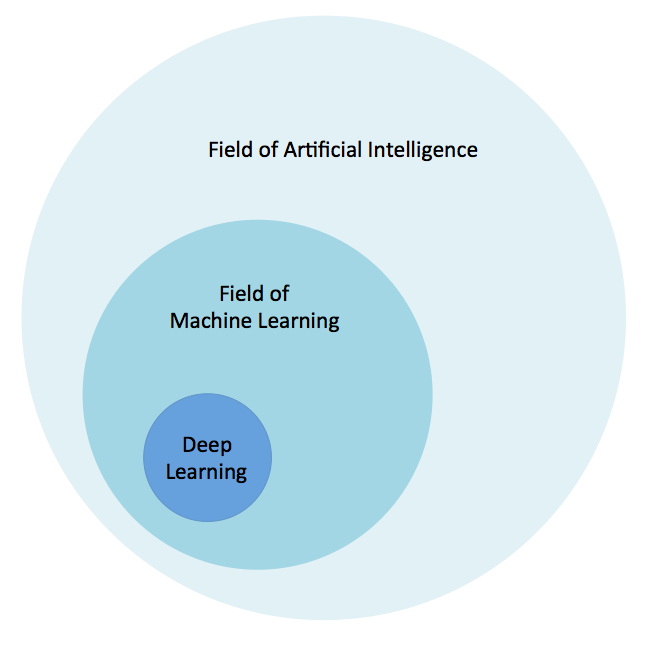
\includegraphics[width=8cm]{figs/ai-ml-dl-relationship.png}
	\caption{Relación entre Inteligencia Artificial, Machine Learning y Deep Learning}
	\label{fig:ai-ml-dl}
\end{figure}

El \textit{Deep Learning} se diferencia del \textit{Machine Learning} convencional, en que están formados por modelos con distintas ramas de procesamiento que son capaces de extraer las representaciones de los datos con varios niveles de abstracción \cite{lecun2015deep}. Mucha de la teoría relacionada se puede encontrar en los años 50 y 60, sin embargo, las aplicaciones y la capacidad de cómputo eran limitadas en la época, hasta ahora donde la capacidad de computación ha crecido a gran escala y en conjunto con las nuevas técnicas propuestas, una mayor cantidad de datos y la aplicación de transformaciones no lineales hacen que esta vertiente viva su época dorada.

Una de las implementaciones más representativas del \textit{Deep Learning} se trata de las redes neuronales, las cuales se encuentran basadas en el funcionamiento del cerebro humano, utilizando el concepto de neuronas que pueden realizar cálculos, la conexión entre las mismas, la función de realizar una tarea específica, etc. Añadir, que se encuentra basado y que el cerebro humano es un sistema mucho más complejo que las redes neuronales y tiene muchos más comportamientos \cite{haykin1994neural}.


Dentro del \textit{Machine Learning}, los algoritmos pueden dividirse según como se realice el entrenamiento del modelo, afectando también a la evaluación y las aplicaciones del mismo. Estas categorias son: \textit{Aprendizaje Supervisado (Supervised Learning), Aprendizaje No Supervidado (Unsupervised Learning) y Aprendizaje Semi-Supervisado (Semi-Supervised Learning)}

\subsection{Aprendizaje Supervisado}

El aprendizaje supervisado se caracteriza por utilizar un conjunto de variables de entrada y encontrar la función que más se aproxime a los valores de salida \cite{Liu2012}. Actualmente es una de las metodologías más utilizadas en \textit{Machine Learning} y es una de las más avanzadas en el campo, sin embargo, la necesidad de los valores de salida (variable dependiente o \textit{target}) requiere que el conjunto de datos se encuentre etiquetado, es decir, para las observaciones de las variables de entrada debe existir la variable de salida para poder general el modelo. En muchos casos este etiquetado se debe de realizar manualmente, por lo que es un proceso que requiere mucho tiempo.

Uno de los modelos más sencillos de aprendizaje supervisado es la regresión lineal (simple), ésta permite ajustar a una serie de puntos conocidos , \textit{x}, y su respuesta \textit{y} \cite{james2013introduction}, generando una función que permite predecir los valores de \textit{y} con valores no conocidos de \textit{x}:

\begin{equation}
y = ax + b 
\end{equation}

En este caso se predicen los nuevos valores utilizando la función ajustada, existen distintos métodos para encontrar la recta que ajusta los puntos, siendo uno de los más utilizados el ajuste por mínimos cuadrados:

\begin{equation}
a = \frac{\sum(x_i – \bar{x}) (y_i – \bar{y})} {\sum(x_i – \bar{x})^2}
\end{equation}

\begin{equation}
b = y – a \bar{x}
\end{equation}

\begin{figure}[H]
	\centering
	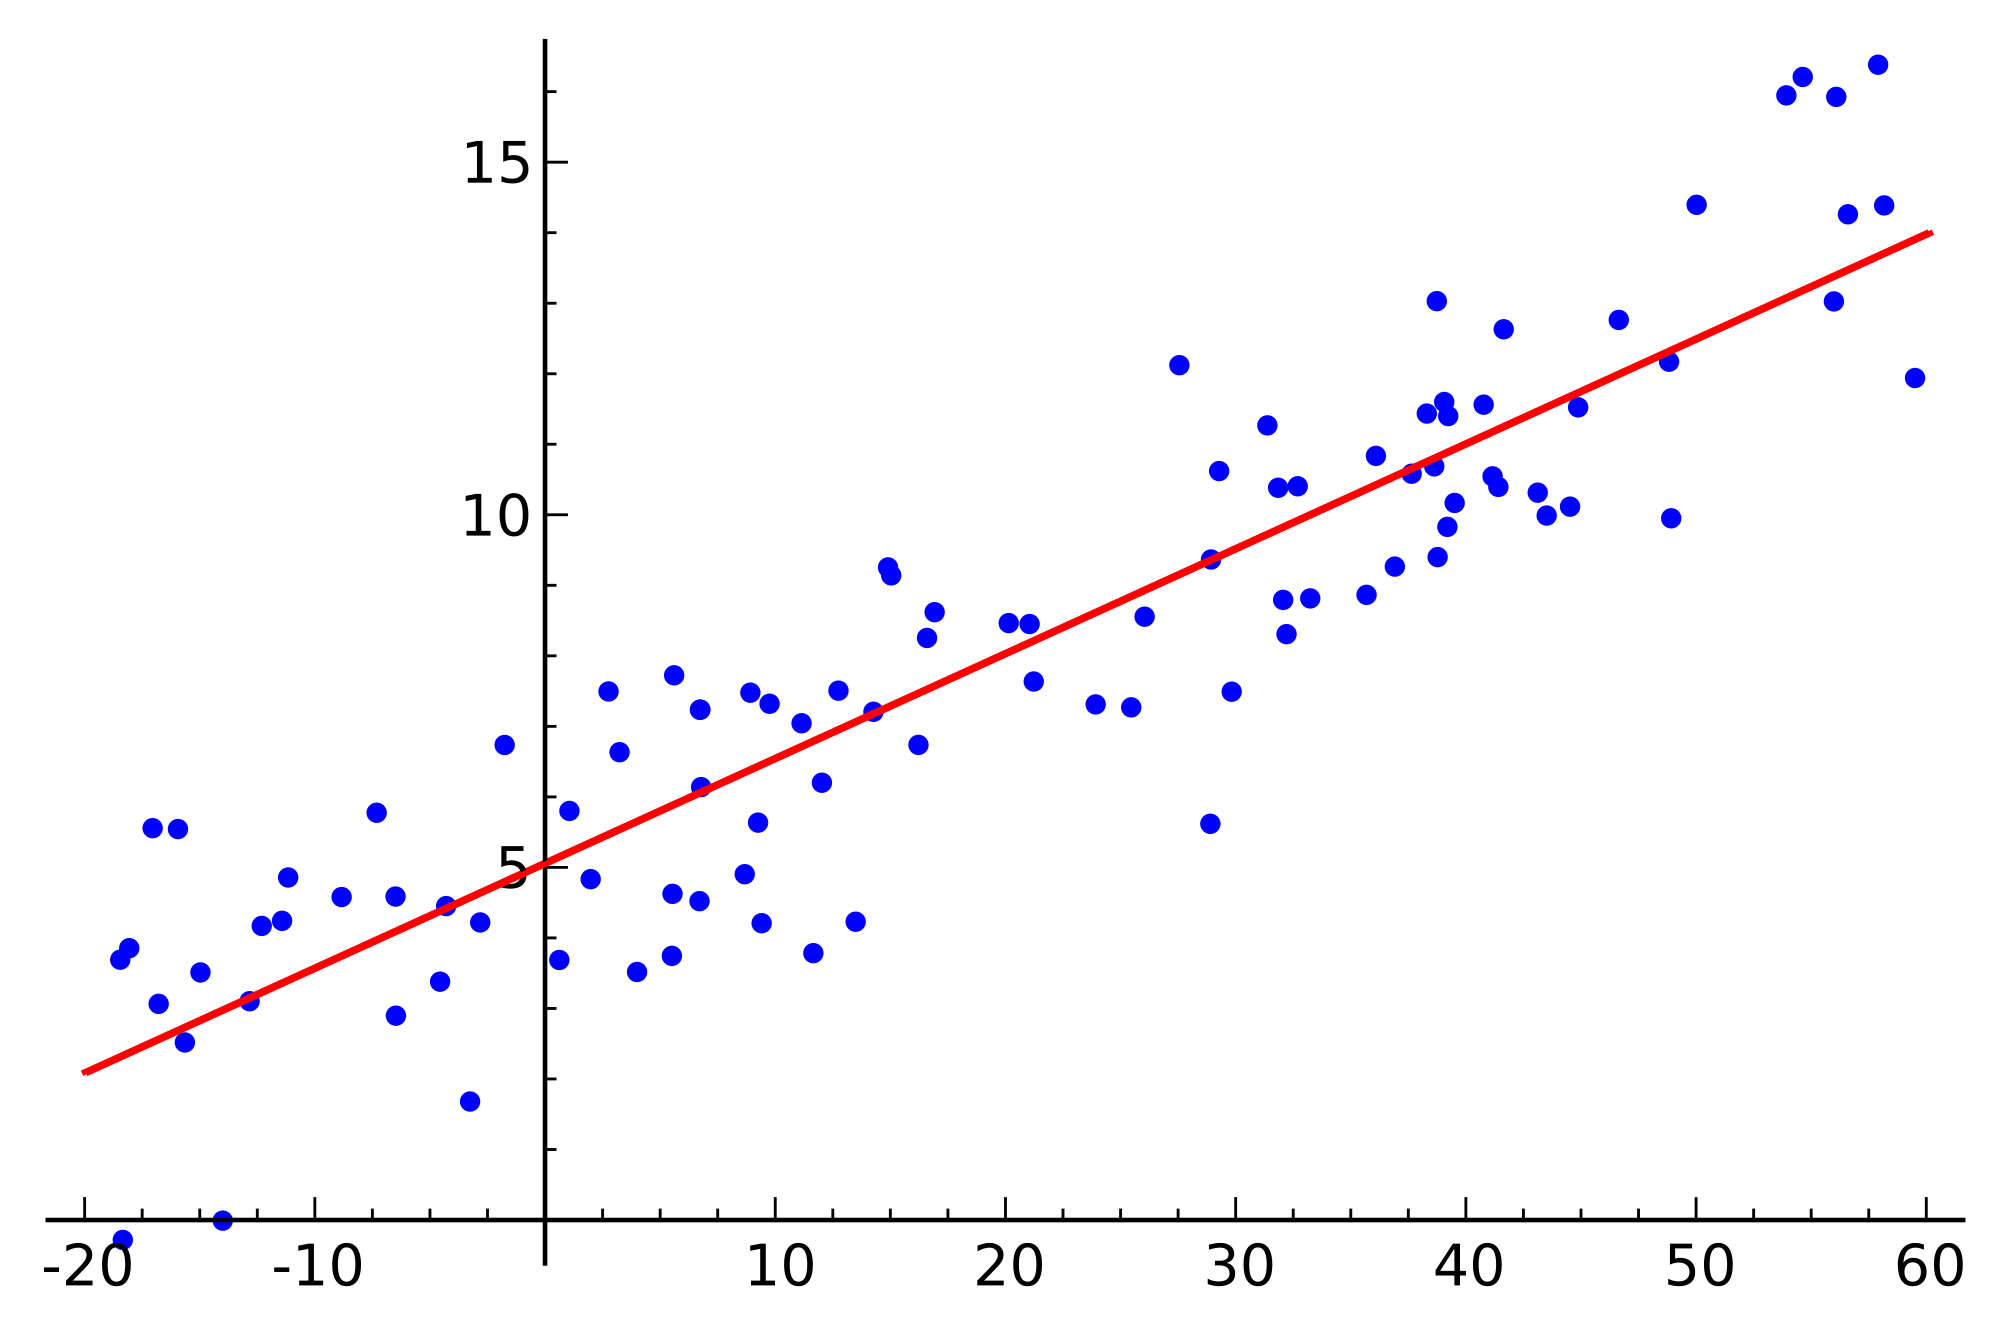
\includegraphics[width=8cm]{figs/Linear_regression.png}
	\caption{Regresión Lineal}
	\label{fig:reglin}
\end{figure}

Como se puede observar en la imagen \ref{fig:reglin}, se ha generado una recta capaz de ajustarse a los puntos y predecir el valor para nuevos puntos. Para generar la función de la recta se ha necesita utilizar la variable dependiente \textit{y} en el entrenamiento para poder generar la función que aproximará los nuevos puntos. 